\section{Optimization problem}
\label{sec:optimization_problem}

As already mentioned in the introduction, the goal of this project is to optimize the hub carrier by maximizing structural stiffness while minimizing mass.

The hub carrier (shown as one of the components in Figure \ref{fig:hub_carrier}) has three main functions:

\begin{itemize}
    \item It closes the kinematic loop made by the two control arms;
    \item It receives the inputs from the steering rod and transfers them to the wheel;
    \item It bears the static and dynamic loads coming from the road and the brake caliper.
\end{itemize}

\begin{figure}[H]
    \centering
    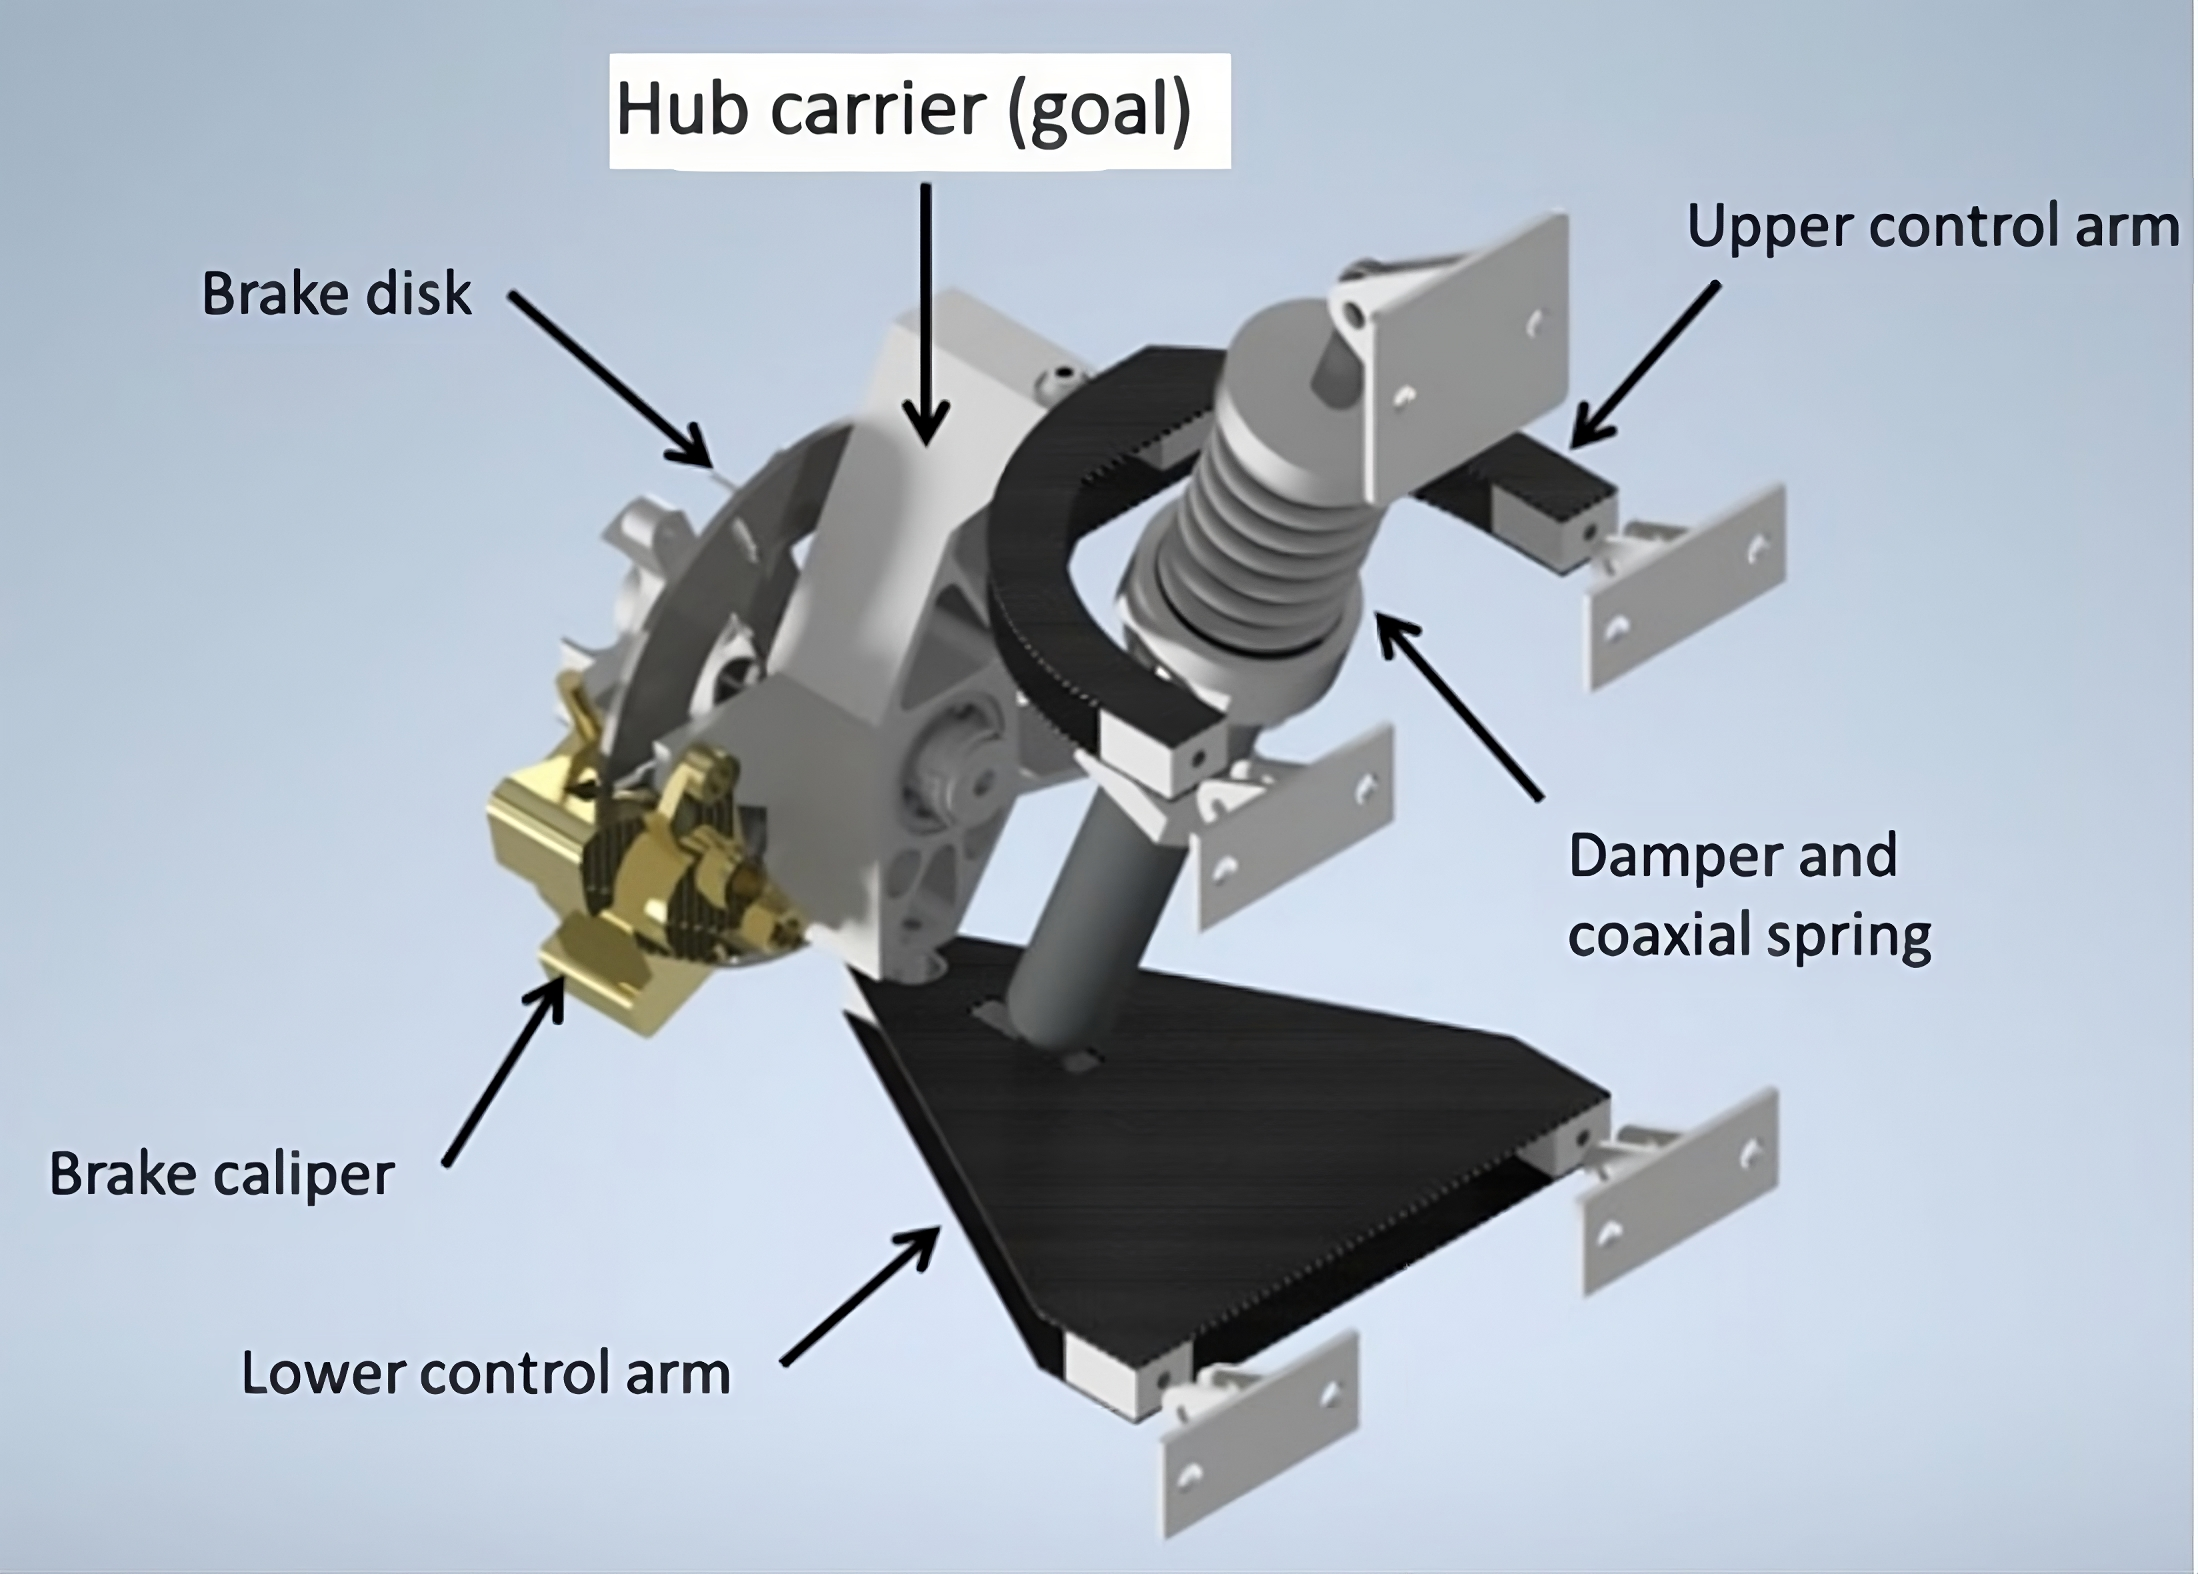
\includegraphics[width=0.7\textwidth]{img/hub_carrier.png}
    \caption{Schematic representation of the front wheel assembly. The hub carrier is indicated by a proper label.}
    \label{fig:hub_carrier}
\end{figure}


\subsection{Design domain}
\label{subsec:design_domain}

As a first approximation, the design domain is defined as the volume enclosed by the hub carrier's outer surface.
This choice is made to simplify the problem and to avoid the definition of complex initial geometries.

\begin{figure}[H]
    \centering
    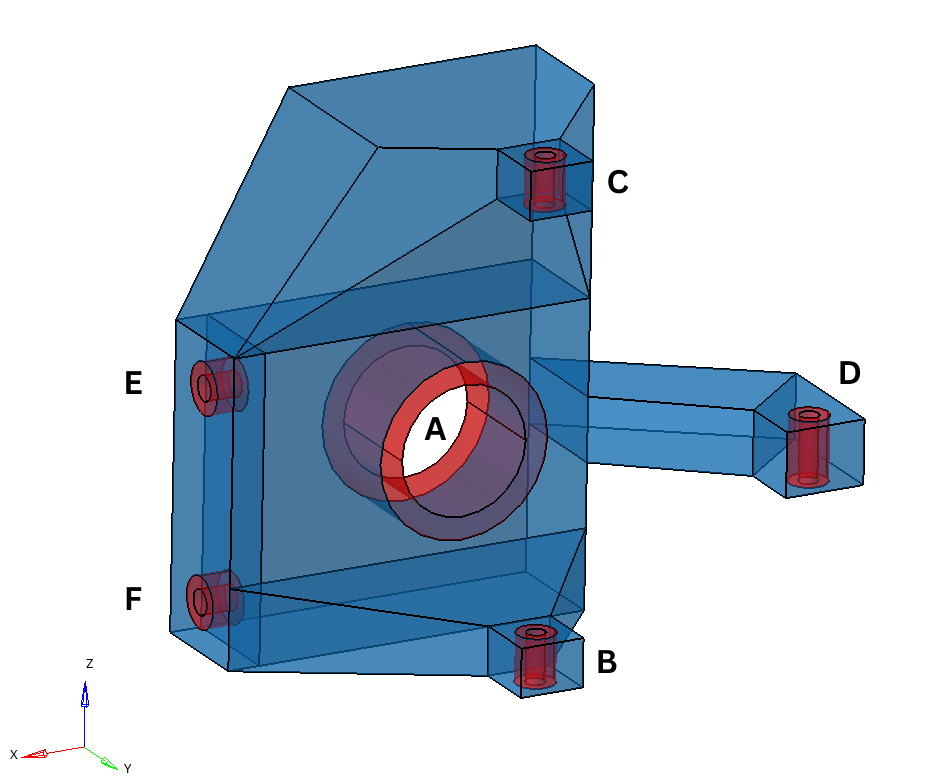
\includegraphics[width=0.7\textwidth]{img/initial_design_domain_labels.png}
    \caption{Initial domain definition.}
    \label{fig:design_domain}
\end{figure}

In Figure \ref{fig:design_domain}, the design domain is shown in blue, while the non-design domain (i.e., the hub carrier's connecting points with the rest of the vehicle) is shown in red.
Connection points are highlighted via the labels $A \dots F$.

The function of each connection point is as follows:

\begin{itemize}
    \item Point $A$: connection with the wheel spindle, all the loads coming from the wheel are transferred to this point;
    \item Point $B$: connection with the lower control arm and the damper, all the vertical loads are transferred to this point;
    \item Point $C$: connection with the upper control arm;
    \item Point $D$: connection with the steering rod;
    \item Points $E$ and $F$: connection with the brake caliper.
\end{itemize}

Based on the function of each connection point, the following boundary conditions are applied to the design domain:

\begin{itemize}
    \item Point $B$: full 3D pin constraint (i.e., free rotation but no translation);
    \item Point $C$: constrained in the $\vec{x}$ and $\vec{y}$ directions;
    \item Point $D$: constrained in the $\vec{y}$ direction;
\end{itemize}


\subsection{Load cases}
\label{subsec:load_cases}

In the following, a brief description of the load cases is provided.

\paragraph{Pure rolling}
The hub carrier is subject only to the vertical load coming from the vehicle's weight. The load is applied at point $A$ and has a magnitude of $F_z = 400 [N]$.

\paragraph{Braking}
Due to the braking action, the load is transferred from the rear to the front axle and a horizontal force is also generated.
Loads are applied to point $A$ with a magnitude of $F_z = 1300 [N]$ and $F_x = -200 [N]$, and points $E$ and $F$ with a magnitude of $F_z = -350 [N]$ each.

\paragraph{Internal turn}
Due to inertia, the vehicle is subject to a lateral acceleration which generates a lateral force on the wheel and a moment on the hub carrier.
Loads are applied to point $A$ with a magnitude of $F_y = -200 [N]$, $F_z = 300 [N]$, $M_x = -60 [Nm]$ and $M_z = 4 [Nm]$.

\paragraph{External turn}
Loads are essentially the same as the internal turn, but with opposite signs, except for the vertical force in $A$ which became $F_z = 500 [N]$.

\paragraph{Internal bump/corners}
In case of a bump or a corner, the wheel is subject to string loads due to high accelerations involved in the phenomena.
We can consider loads applied to point $A$ with a magnitude of $F_x = 500 [N]$, $F_y = 500 [N]$, $F_z = 1000 [N]$ and $M_x = 150 [Nm]$.

\paragraph{External bump/corners}
Loads are essentially the same as the internal bump/corners, but with opposite signs, except for the vertical force in $A$ that remains $F_z = 1000 [N]$.


\subsection{Material properties}
\label{subsec:material_properties}

In order to minimize the mass of the hub carrier, the material choice has to be carefully made.
In particular, the use of steel is not recommended due to its high density which would lead to a heavy component.

For this reason, the material chosen is \textit{Aluminum 6061 T6}, which has a density of $\rho = 2700 [kg/m^3]$ and a Young's modulus of $E = 70 [GPa]$.
The yield strength is $\sigma_{\text{YS}} = 275 [MPa]$ and the Poisson's ratio is $\nu = 0.33$.


\subsection{Objectives and constraints}
\label{subsec:objectives_constraints}

The formal definition of the topology optimization problem can be given as the minimization of the weighted compliance $C$ for the six load cases described in Section \ref{subsec:load_cases} subjected to the following constraints:

\begin{itemize}
    \item Camber stiffness: $K_c \geq 160\cdot10^3 [Nm/rad]$;
    \item Toe stiffness: $K_t \geq 84\cdot10^3 [Nm/rad]$;
    \item Mass fraction: $m_{opt} \leq 0.225 \cdot m_0$;
    \item Manufacturing constraints: constant cross-sections along the $\vec{y}$ direction (i.e., extrusion like shapes).
\end{itemize}

The optimization variables are the density of each element in the design domain, which can vary between 0 (void) and 1 (solid).
